The \textit{Experiment Management} module is responsible for the creation of an
experiment with all it's associated jobs based on the specifications submitted
by the user such as the algorithms, datasets, type of measurements, probe 
interval and number of iterations that should be performed. 

This module further is responsible for communication with the message bus to
place job requests on a queue, retrieve results from finished jobs and process
the heartbeat messages of monitor nodes.

A further responsibility of this module includes also the retrieving of results
about a specified job.



\subsection{Scope}
The scope for the Experiment Management Service module is shown in Figure \ref{fig:experimentManagementScope}.
\begin{figure}[H]
  \begin{center}
  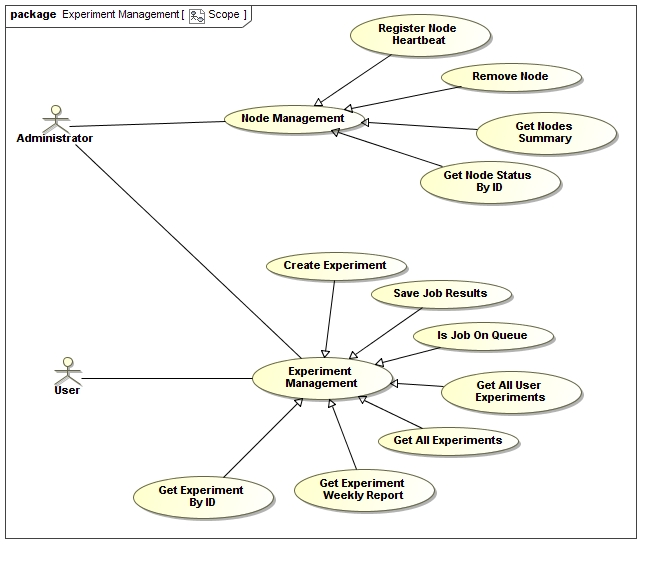
\includegraphics[scale=0.38]{../Diagrams and Charts/Experiment/Scope.jpg}
  \caption{Experiment Management Scope}
  \label{fig:experimentManagementScope}
  \end{center}
\end{figure}



\subsection{Domain Model}
The domain model for the Experiment Management Service module is shown in Figure \ref{fig:experimentManagementDomain}.
\begin{figure}[H]
  \begin{center}
  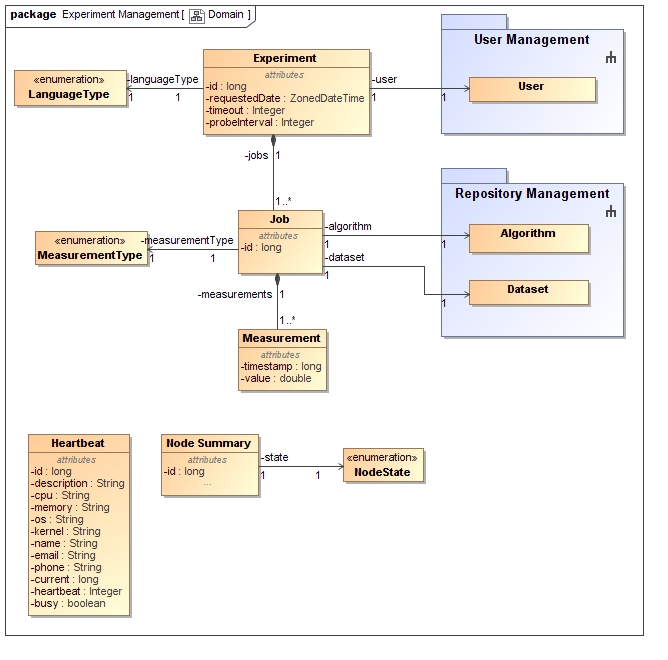
\includegraphics[scale=0.38]{../Diagrams and Charts/Experiment/Domain.jpg}
  \caption{Experiment Management Domain Model}
  \label{fig:experimentManagementDomain}
  \end{center}
\end{figure}



\subsection {Create Experiment}
The \textit{Create Experiment} use case is concerned with creation of an
experiment and its associated jobs specified by the supplied parameters. Upon
creation the jobs will be placed at some pre-arranged location for monitor nodes
to find.

\subsubsection{Service Contract}
The service contract for creating an experiment is shown in 
Figure \ref{fig:createExperimentServiceContract}.
\begin{figure}[H]
  \begin{center}
  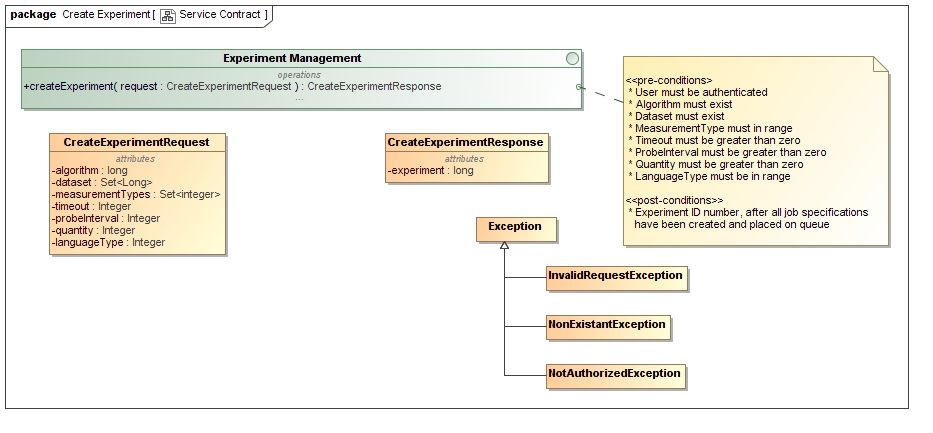
\includegraphics[scale=0.38]{../Diagrams and Charts/Experiment/Create Experiment Service Contract.jpg}
  \caption{Create Experiment Service Contract}
  \label{fig:createExperimentServiceContract}
  \end{center}
\end{figure}

The use case creates a new experiment object as well as the associated jobs from
the supplied parameters. The use case will match each algorithm and dataset to a
measurement type. Such a matching constitutes one job for a set of parameters, 
after which a total of N jobs will be created for one such matching, where N is
specified by the user quantity parameter.

For a user to create an experiment the following must hold true:
\begin{itemize}
  \item The user must be authenticated.
  \item The algorithm and dataset must refer to valid objects in the back end.
  \item The measurement and language types must be a valid types.
  \item The probe interval, timeout and quantity values must be greater than zero.
  \item The probe interval must be less than the timeout interval.
\end{itemize}

\subsubsection {Functional Requirements}
The lower level services required by the create experiment service to 
either check the pre-conditions or address the post-conditions is shown in
Figure \ref{fig:createExperimentFunctionalRequirements}.

Note that the create experiment service is responsible for randomizing the order
of the jobs and placing them at the pre-arranged location for the monitor nodes
to find. The other services 
\begin{itemize}
  \item retrieving the required objects and files to be sent along to the monitor
        nodes
  \item persist the experiment and jobs
\end{itemize}
\begin{figure}[H]
  \begin{center}
  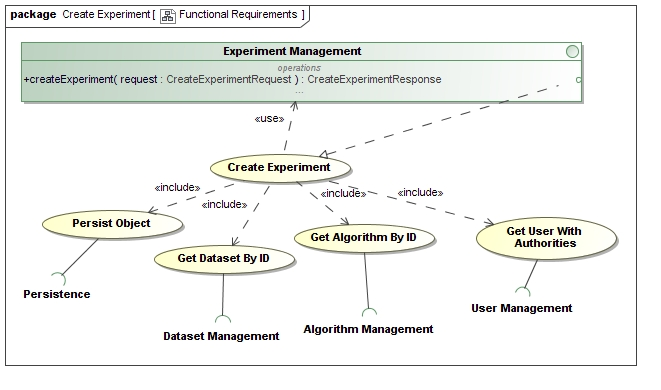
\includegraphics[scale=0.38]{../Diagrams and Charts/Experiment/Create Experiment Functional Requirements.jpg}
  \caption{Create Experiment Functional Requirements}
  \label{fig:createExperimentFunctionalRequirements}
  \end{center}
\end{figure}



\subsection {Get All Experiments}
The \textit{Get All Experiments} use case is concerned with retrieving a list
of all experiments from the persistence provider.

\subsubsection{Service Contract}
The service contract for retrieving all experiments is shown in 
Figure \ref{fig:getAllExperimentsServiceContract}.
\begin{figure}[H]
  \begin{center}
  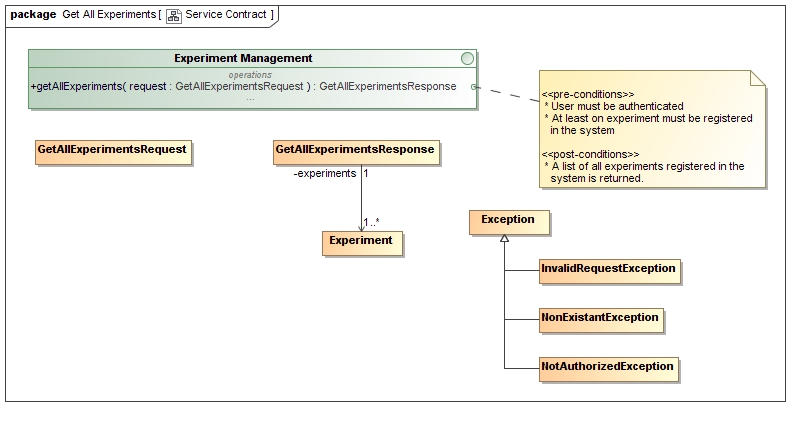
\includegraphics[scale=0.38]{../Diagrams and Charts/Experiment/Get All Experiments Service Contract.jpg}
  \caption{Get All Experiments Service Contract}
  \label{fig:getAllExperimentsServiceContract}
  \end{center}
\end{figure}



\subsection {Get All User Experiments}
The \textit{Get All User Experiments} use case is concerned with retrieving a
list of all experiments related to the user in the current security context.

\subsubsection{Service Contract}
The service contract for retrieving all experiments for the currently logged-in
user is shown in Figure \ref{fig:getAllUserExperimentsServiceContract}.
\begin{figure}[H]
  \begin{center}
  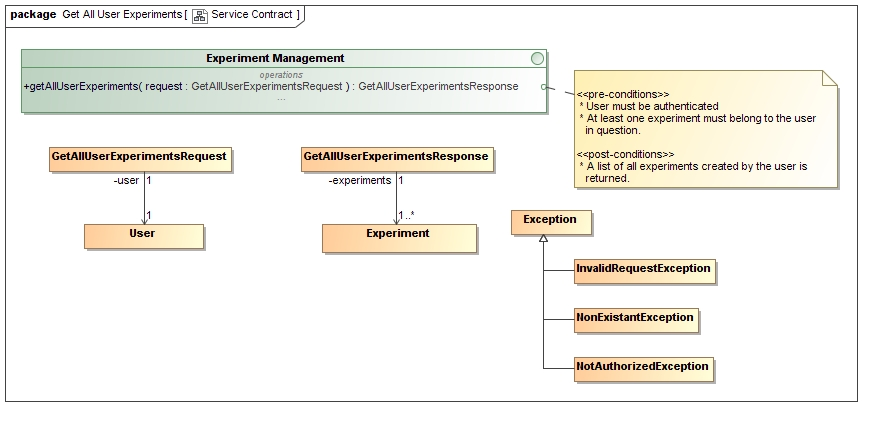
\includegraphics[scale=0.38]{../Diagrams and Charts/Experiment/Get All User Experiments Service Contract.jpg}
  \caption{Get All User Experiments Service Contract}
  \label{fig:getAllUserExperimentsServiceContract}
  \end{center}
\end{figure}

\subsubsection {Functional Requirements}
The lower level services required by the get all user experiments service to 
either check the pre-conditions or address the post-conditions is shown in
Figure \ref{fig:getAllUserExperimentsFunctionalRequirements}.
\begin{figure}[H]
  \begin{center}
  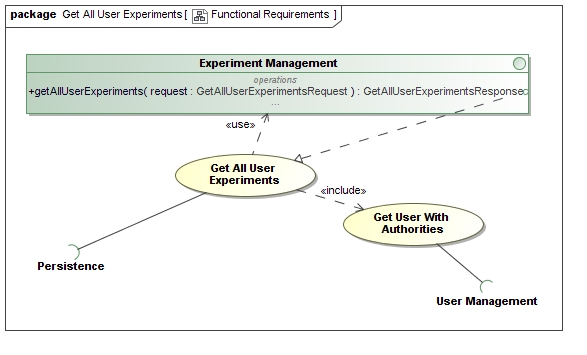
\includegraphics[scale=0.38]{../Diagrams and Charts/Experiment/Get All User Experiments Functional Requirements.jpg}
  \caption{Get All User Experiments Functional Requirements}
  \label{fig:getAllUserExperimentsFunctionalRequirements}
  \end{center}
\end{figure}



\subsection {Get Experiment By ID}
The \textit{Get Experiment By ID} use case is concerned with retrieving an
experiment based on its ID number.

\subsubsection{Service Contract}
The service contract for retrieving an experiment by its ID number is show in
Figure \ref{fig:getExperimentByIDServiceContract}.
\begin{figure}[H]
  \begin{center}
  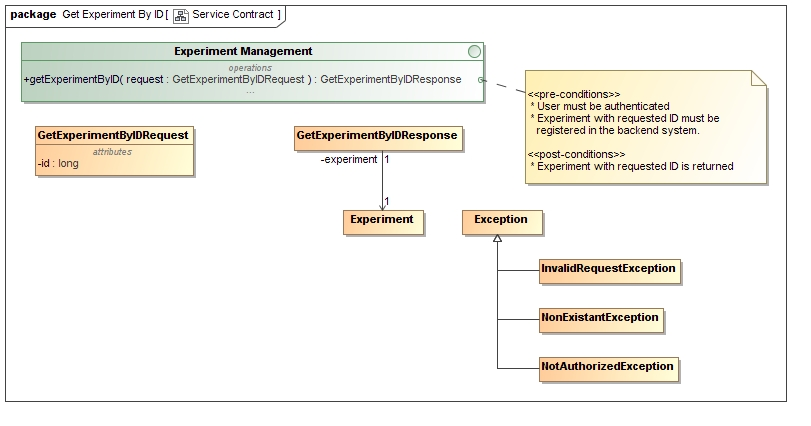
\includegraphics[scale=0.38]{../Diagrams and Charts/Experiment/Get Experiment By ID Service Contract.jpg}
  \caption{Get Experiment By ID Service Contract}
  \label{fig:getExperimentByIDServiceContract}
  \end{center}
\end{figure}



\subsection {Get Experiment Weekly Report}
The \textit{Get Experiment Weekly Report} use case is concerned with retrieving
a range of metrics for all experiments done on the the benchmarking system over
the last week (7 days).

\subsubsection{Service Contract}
The service contract for retrieving the weekly metrics of the management system
is shown in Figure \ref{fig:getExperimentWeeklyReportServiceContract}.
\begin{figure}[H]
  \begin{center}
  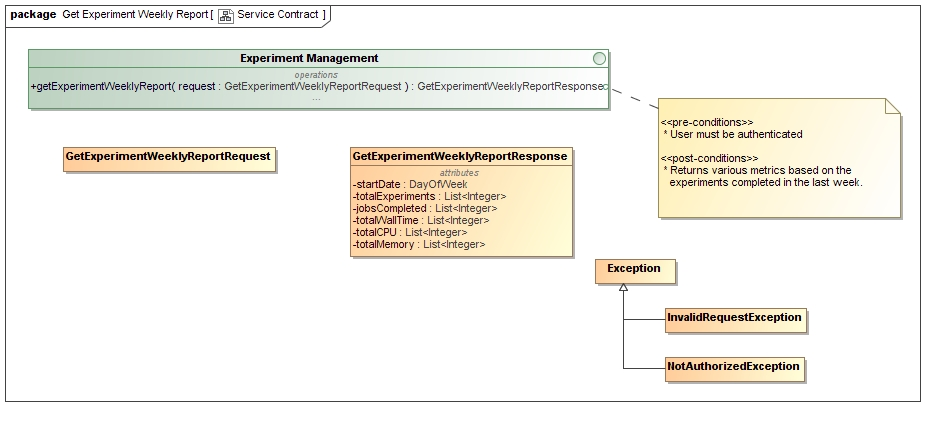
\includegraphics[scale=0.38]{../Diagrams and Charts/Experiment/Get Experiment Weekly Report Service Contract.jpg}
  \caption{Get Experiment Weekly Report Service Contract}
  \label{fig:getExperimentWeeklyReportServiceContract}
  \end{center}
\end{figure}

\subsubsection {Functional Requirements}
The lower level services required by the get experiment weekly report service to 
either check the pre-conditions or address the post-conditions is shown in
Figure \ref{fig:getExperimentWeeklyReportFunctionalRequirements}.
\begin{figure}[H]
  \begin{center}
  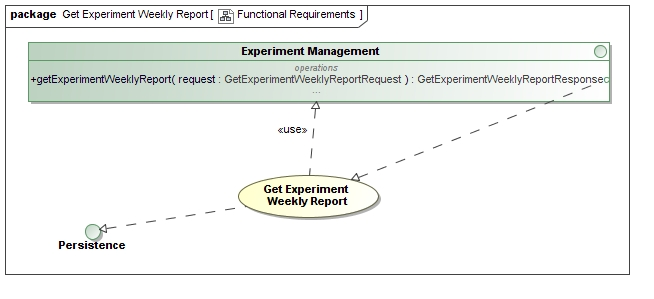
\includegraphics[scale=0.38]{../Diagrams and Charts/Experiment/Get Experiment Weekly Report Functional Requirements.jpg}
  \caption{Get Experiment Weekly Report Functional Requirements}
  \label{fig:getExperimentWeeklyReportFunctionalRequirements}
  \end{center}
\end{figure}



\subsection {Get Node Status By ID}
The \textit{Get Node Status By ID} use case is concerned with retrieving
the information, for a node identified by its ID number, currently stored in the
monitoring system.

\subsubsection{Service Contract}
The service contract for retrieving the node information from the monitoring system
is shown in Figure \ref{fig:getNodeStatusByIDServiceContract}.
\begin{figure}[H]
  \begin{center}
  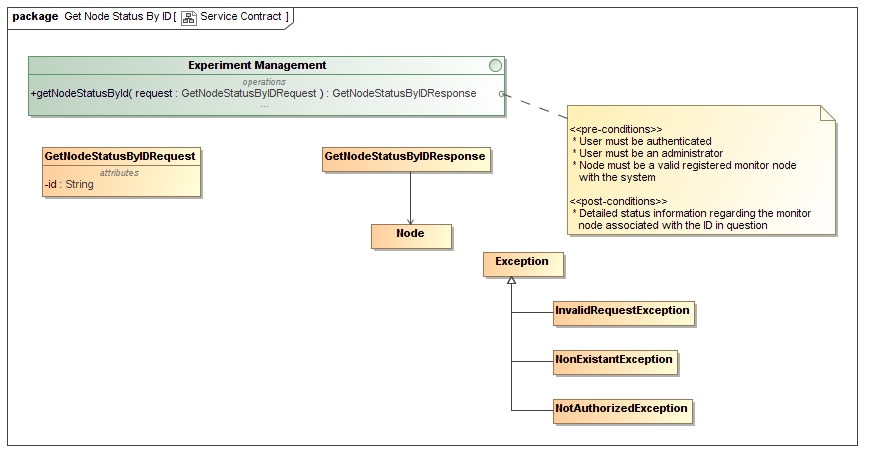
\includegraphics[scale=0.38]{../Diagrams and Charts/Experiment/Get Node Status By ID Service Contract.jpg}
  \caption{Get Node Status By ID Service Contract}
  \label{fig:getNodeStatusByIDServiceContract}
  \end{center}
\end{figure}

\subsubsection {Functional Requirements}
The lower level services required by the get node status by ID service to 
either check the pre-conditions or address the post-conditions is shown in
Figure \ref{fig:getNodeStatusByIDFunctionalRequirements}.
\begin{figure}[H]
  \begin{center}
  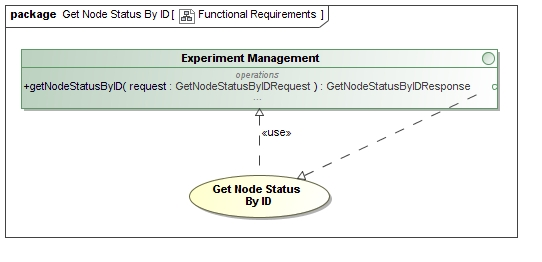
\includegraphics[scale=0.38]{../Diagrams and Charts/Experiment/Get Node Status By ID Functional Requirements.jpg}
  \caption{Get Node Status By ID Functional Requirements}
  \label{fig:getNodeStatusByIDFunctionalRequirements}
  \end{center}
\end{figure}



\subsection {Is Job On Queue}
The \textit{Is Job On Queue} use case is concerned with identifying if a job is
currently still waiting on the queue to be processed, or if it is done being
processed and hence have a list of measurements.

\subsubsection{Service Contract}
The service contract for checking if a specified job is still on the queue is
shown in Figure \ref{fig:isJobOnQueueServiceContract}.
\begin{figure}[H]
  \begin{center}
  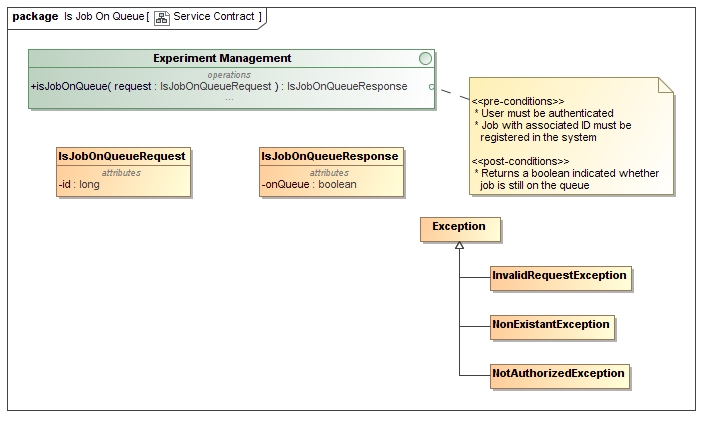
\includegraphics[scale=0.38]{../Diagrams and Charts/Experiment/Is Job On Queue Service Contract.jpg}
  \caption{Is Job On Queue Service Contract}
  \label{fig:isJobOnQueueServiceContract}
  \end{center}
\end{figure}



\subsection {Register Node Heartbeat}
The \textit{Register Node Heartbeat} use case is concerned with registering
the heartbeat of a monitor node with the monitoring system. This use case
is used to both register new nodes and to refresh currently registered nodes.

\subsubsection{Service Contract}
The service contract for registering the heartbeat of a monitor node with the
management system is shown in Figure \ref{fig:registerNodeHeartbeatServiceContract}.
\begin{figure}[H]
  \begin{center}
  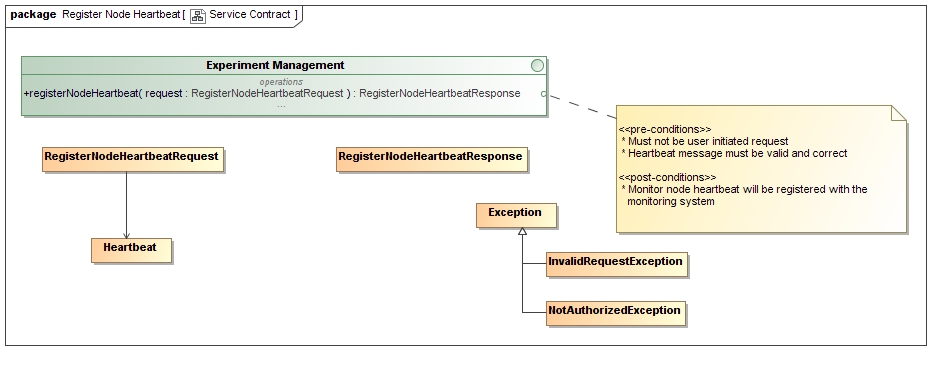
\includegraphics[scale=0.38]{../Diagrams and Charts/Experiment/Register Node Heartbeat Service Contract.jpg}
  \caption{Register Node Heartbeat Service Contract}
  \label{fig:registerNodeHeartbeatServiceContract}
  \end{center}
\end{figure}

\subsubsection {Functional Requirements}
The lower level services required by the register node heartbeat service to 
either check the pre-conditions or address the post-conditions is shown in
Figure \ref{fig:registerNodeHeartbeatFunctionalRequirements}.
\begin{figure}[H]
  \begin{center}
  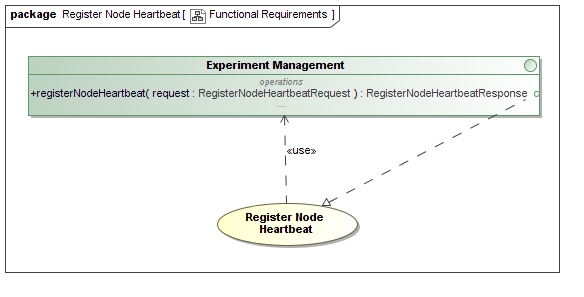
\includegraphics[scale=0.38]{../Diagrams and Charts/Experiment/Register Node Heartbeat Functional Requirements.jpg}
  \caption{Register Node Heartbeat Functional Requirements}
  \label{fig:registerNodeHeartbeatFunctionalRequirements}
  \end{center}
\end{figure}



\subsection {Remove Node}
The \textit{Remove Node} use case is concerned with removing a node from the
monitoring system. Note that if the nodes continues to send heartbeat messages,
the node will be re-registered in the system. This is to ensure a loose-coupling
with the back end management system and the monitor nodes themselves that should
remain totally autonomous and ephemeral.

\subsubsection{Service Contract}
The service contract for removing a registered monitor node from the back end 
system is shown in Figure \ref{fig:removeNodeServiceContract}.
\begin{figure}[H]
  \begin{center}
  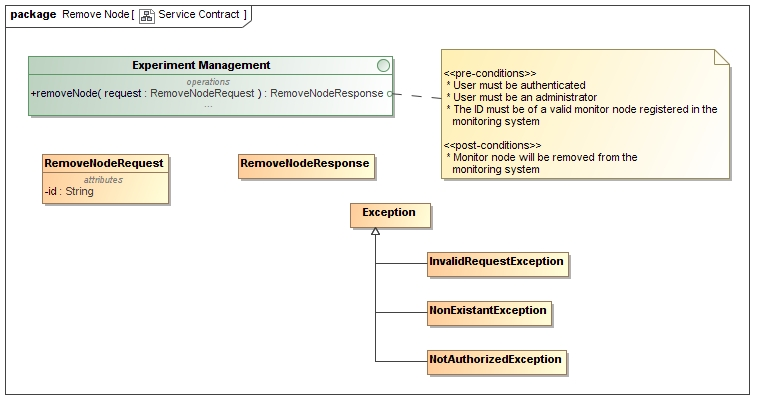
\includegraphics[scale=0.38]{../Diagrams and Charts/Experiment/Remove Node Service Contract.jpg}
  \caption{Remove Node Service Contract}
  \label{fig:removeNodeServiceContract}
  \end{center}
\end{figure}

\subsubsection {Functional Requirements}
The lower level services required by the remove node service to 
either check the pre-conditions or address the post-conditions is shown in
Figure \ref{fig:removeNodeFunctionalRequirements}.
\begin{figure}[H]
  \begin{center}
  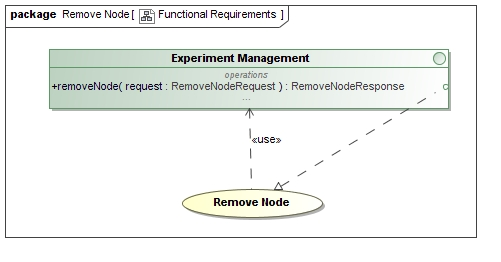
\includegraphics[scale=0.38]{../Diagrams and Charts/Experiment/Remove Node Functional Requirements.jpg}
  \caption{Remove Node Functional Requirements}
  \label{fig:removeNodeFunctionalRequirements}
  \end{center}
\end{figure}



\subsection {Save Job Results}
The \textit{Save Job Results} use case is concerned with removing results from a
pre-arranged central location with the monitor nodes and attaching the results
to the experiment in the back end.

\subsubsection{Service Contract}
The service contract for retrieving the saving the results for a job is shown 
Figure \ref{fig:saveJobResultsServiceContract}.
\begin{figure}[H]
  \begin{center}
  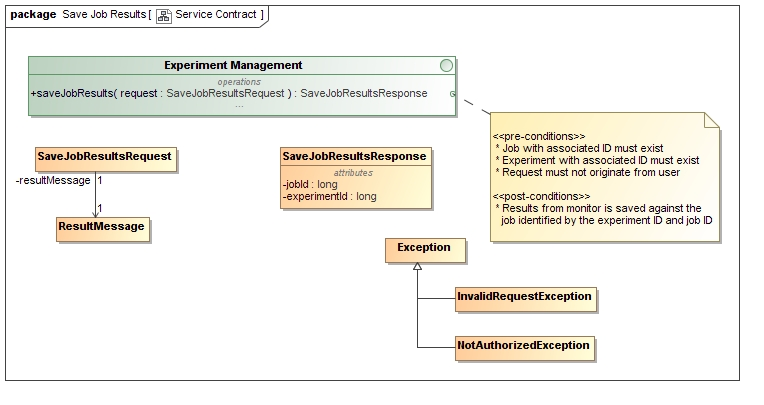
\includegraphics[scale=0.38]{../Diagrams and Charts/Experiment/Save Job Results Service Contract.jpg}
  \caption{Save Job Results Service Contract}
  \label{fig:saveJobResultsServiceContract}
  \end{center}
\end{figure}
